\section{Experiments}
\label{sec:experiments}

Our experimental analysis addresses five questions:
(1) How does CORELS' accuracy compare to other algorithms?
(2) How does CORELS' model size compare to other algorithms?
(3) How rapidly does the objective function converge?
(4) How rapidly does CORELS prune the search space?
(5) How much does each of the implementation optimizations contribute to CORELS' performance?

All results that we present were executed on a server with two Intel Xeon E5-2699~v4
(55~MB cache, 2.20~GHz) processors and 448~GB RAM.
%
Except where we mention a memory constraint, all experiments
can run comfortably on smaller machines, \eg a laptop with 16GB~RAM.

Our evaluation focuses on two socially-important prediction problems associated
with recent, publicly-available datasets:
\begin{itemize}
\item Predicting which individuals in the ProPublica COMPAS
dataset~\citep{LarsonMaKiAn16} recidivate within two years.
The dataset contains records for 7,215 individuals.
%
\item Using the NYCLU 2014 stop-and-frisk dataset~\citep{nyclu:2014} to predict
whether a weapon will be found on a stopped individual who is frisked or searched.
%
From the original dataset of 45,787 records, each describing an incident involving
a stopped person, we identify a subset of 29,595 records for which the individual
was frisked and/or searched (Appendix~C).
%
Of these, criminal possession of a weapon was identified in about only 5\% of instances.
%
To address the class imbalance for this problem,  we sample records from the
smaller class with replacement; in our 10-fold cross-validation experiments,
each fold contains 50,743 datapoints.~\footnote{We generate cross-validation folds fist,
and then resample within each fold.}
\end{itemize}
%
Our choice of and approach to the second problem is inspired by the work
of~\citet{Goel16}, who develop regression models to analyze racial disparities
in New York City's stop-and-frisk policy, for a similar, larger dataset.
%
In particular, the authors arrive at a simple and interpretable heuristic that
could potentially help police officers more effectively decide when to
frisk and/or search stopped individuals, \ie when such
interventions are likely to discover criminal possession of a weapon.

We first ran a 10-fold cross validation experiment using CORELS
and eight other algorithms:
logistic regression, support vector machines, AdaBoost, CART, C4.5,
random forests, RIPPER, and scalable Bayesian rule lists (SBRL).~\footnote{For
SBRL, we use the C implementation at \url{https://github.com/Hongyuy/sbrlmod}.}
%
We use standard R packages, with default parameter settings,
for the first seven algorithms.~\footnote{For CART, C4.5 (J48), and RIPPER,
\ie the tree and rule list learning algorithms, we use the implementations
from the R packages rpart, RWeka, and caret, respectively.
%
By default, CART uses complexity parameter ${cp = 0.01}$,
and C4.5 uses complexity parameter ${C = 0.25}$.
}

\begin{figure}[t]
\begin{algorithmic}
\State \bif $(age = 23-25) \band (priors = 2-3)$ \bthen $yes$
\State \belif $(age = 18-20)$ \bthen $yes$
\State \belif $(sex = male) \band (age = 21-22)$ \bthen $yes$
\State \belif $(priors > 3)$ \bthen $yes$
\State \belse $no$
\end{algorithmic}
\vspace{1mm}
\begin{algorithmic}
\State \bif $(age = 23-25) \band (priors = 2-3)$ \bthen $yes$
\State \belif $(age = 18-20)$ \bthen $yes$
\State \belif $(priors > 3)$ \bthen $yes$
\State \belif $(sex = male) \band (age = 21-22)$ \bthen $yes$
\State \belse $no$
\end{algorithmic}
\vspace{1mm}
\begin{algorithmic}
\State \bif $(age = 23-25) \band (priors = 2-3)$ \bthen $yes$
\State \belif $(sex = male) \band (age = 21-22)$ \bthen $yes$
\State \belif $(age = 18-20)$ \bthen $yes$
\State \belif $(priors > 3)$ \bthen $yes$
\State \belse $no$
\end{algorithmic}
\caption{Example optimal rule lists that predict two-year recidivism for the
ProPublica dataset, found by CORELS, across 10 cross-validation folds.
%
The most common rule list was found by 6 folds (top),
the next was found by 2 folds (middle), and the last by 1 fold (bottom).
%
We observe that all of these rule lists start with the same rule,
end with the same default rule, and contain the same prefix rules, up to a permutation;
the prefix rules always predict the positive class label,
and the default rule always predicts the negative class label.
%
Note that our objective does is not designed to enforce any of these properties,
though some may be seen as desirable.
}
\label{fig:recidivism-all-folds}
\end{figure}

\begin{figure}[t!]
\begin{algorithmic}
\State \bif $(location = transit~authority)$ \bthen $yes$
\State \belif $(stop~reason = suspicious~object)$ \bthen $yes$
\State \belif $(stop~reason = suspicious~bulge)$ \bthen $yes$
\State \belse $no$
\end{algorithmic}
\caption{An example rule list that predicts whether a weapon will be found on a
stopped individual who is frisked or searched, for the NYCLU stop-and-frisk dataset.
%
This is the most common optimal rule list found by CORELS across 10 cross-validation
folds; the others contain the same rules, up to a permutation.
}
\label{fig:weapon-rule-list}
\end{figure}

\begin{figure}[t!]
\begin{center}
%\includegraphics[width=0.75\textwidth]{figs/sketch-comparison.png}
% left lower right upper
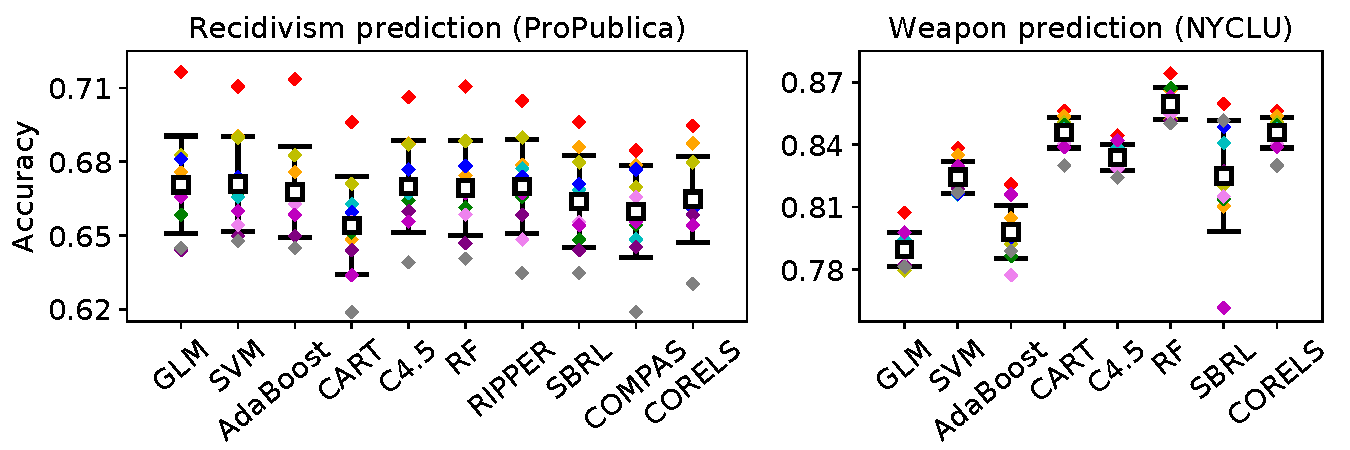
\includegraphics[trim={10mm, 10mm, 25mm, 5mm},
width=0.95\textwidth]{figs/compare-compas-weapon.pdf}
\end{center}
\caption{Comparison of CORELS and a panel of eight other algorithms:
logistic regression~(GLM), support vector machines~(SVM),
AdaBoost, CART, C4.5, random forests~(RF), RIPPER,
scalable Bayesian rule lists~(SBRL).
%
Test accuracy means (white squares),
standard deviations (error bars),
and values (colors correspond to folds),
for 10-fold cross-validation experiments.
%
Left:~Two-year recidivism prediction for the ProPublica COMPAS dataset.
%
For CORELS, we use regularization parameter~${\Reg=0.005}$.
%
Right:~Weapon prediction for the NYCLU stop-and-frisk dataset.
%
For CORELS, we use~${\Reg=0.01}$.
%
Note that we were unable to execute RIPPER for the NYCLU problem.
}
\label{fig:comparison}
\end{figure}

Figures~\ref{fig:recidivism-all-folds} and~\ref{fig:weapon-rule-list}
show example optimal rule lists that CORELS learns
for the ProPublica and NYCLU datasets, respectively.
%
While our goal is to provide illustrative examples, and not to provide a
detailed analysis nor to advocate for the use of these specific models,
we note that these rule lists are short and easy to understand.
%
In particular, the three-rule list for weapon prediction
in Figure~\ref{fig:weapon-rule-list} has the spirit of the heuristic
strategy presented by~\citet{Goel16} that combines three stop criteria
and is based on a reduced version of their full regression model.

Figure~\ref{fig:comparison} shows that there were no statistically significant
differences in algorithm accuracies.
In fact, the difference between folds was far larger than the difference
between algorithms.
We conclude that CORELS produces models whose accuracy is comparable
to those found via other algorithms.

\begin{figure}[t!]
\begin{center}
%\includegraphics[width=0.75\textwidth]{figs/sketch-comparison.png}
% left lower right upper
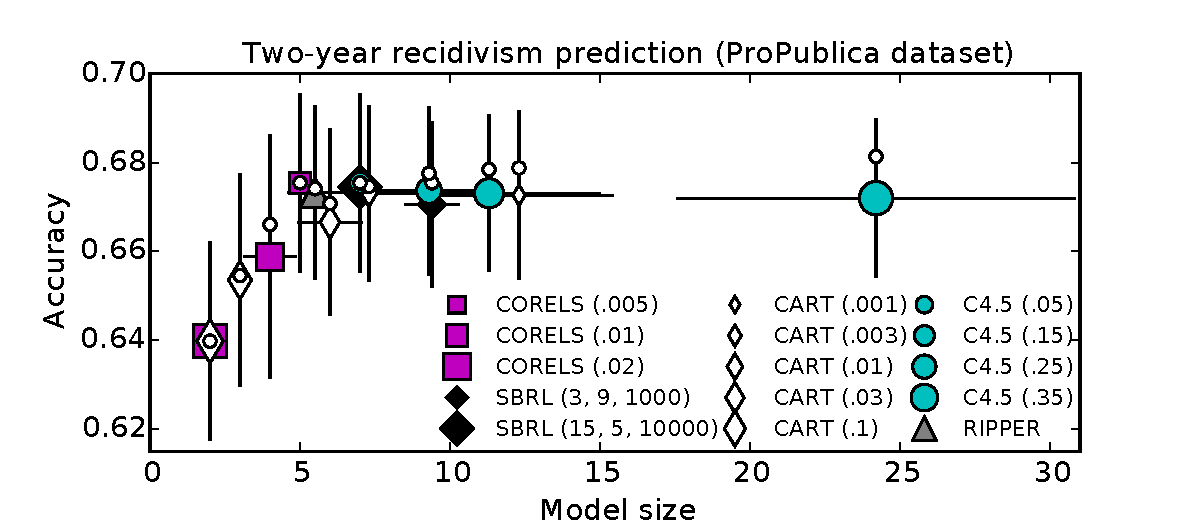
\includegraphics[trim={12mm, 0mm, 24mm, 5mm},
width=0.68\textwidth]{figs/compas-sparsity-training.pdf}
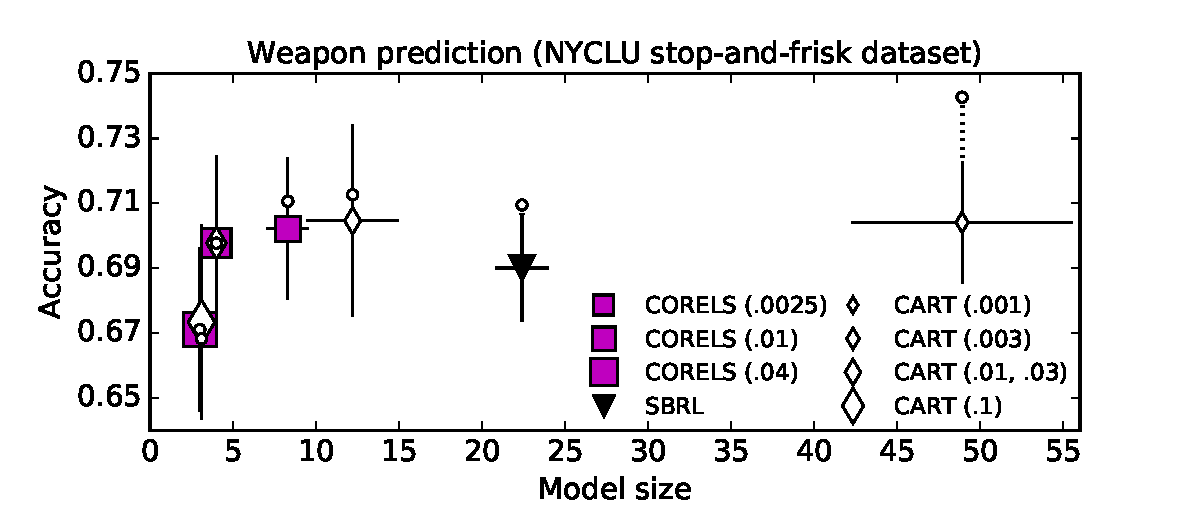
\includegraphics[trim={12mm, 5mm, 24mm, 1mm},
width=0.68\textwidth]{figs/frisk-sparsity-training.pdf}
\end{center}
\caption{Training and test accuracy as a function of model size.
%
For CORELS, CART, and C4.5, we vary the regularization parameter~$\Reg$,
and complexity parameters~$cp$ and~$C$, respectively;
numbers within parentheses in the legend indicate parameter values.
%
Note that the CART implementation sets ${cp = 0.01}$ by default,
and C4.5 uses ${C = 0.25}$.
%
Legend markers and error bars indicate means and standard deviations,
respectively, of test accuracy across cross-validation folds.
%
Small circles mark associated training accuracy means.
%
Top:  Two-year recidivism prediction for the ProPublica COMPAS dataset.
%
None of the models exhibit significant overfitting --
mean training accuracy never exceeds mean test accuracy
by more than about 0.01.
%
Bottom:  Weapon prediction for the NYCLU stop-and-frisk dataset.
%
Only CART with ${cp = 0.001}$ significantly overfits.
%
We do not depict C4.5, which finds large models (${>100}$ leaves)
and dramatically overfits for all tested parameters.
}
\label{fig:sparsity}
\end{figure}

Figure~\ref{fig:sparsity} summarizes differences in accuracy and model size
for CORELS and other tree (CART, C4.5) and rule list (RIPPER, SBRL) learning algorithms.
%
For both problems, CORELS can learn short rule lists without sacrificing accuracy.

\begin{figure}[t!]
\begin{center}
%\includegraphics[width=0.65\textwidth]{figs/sketch-objective.png}
% left lower right upper
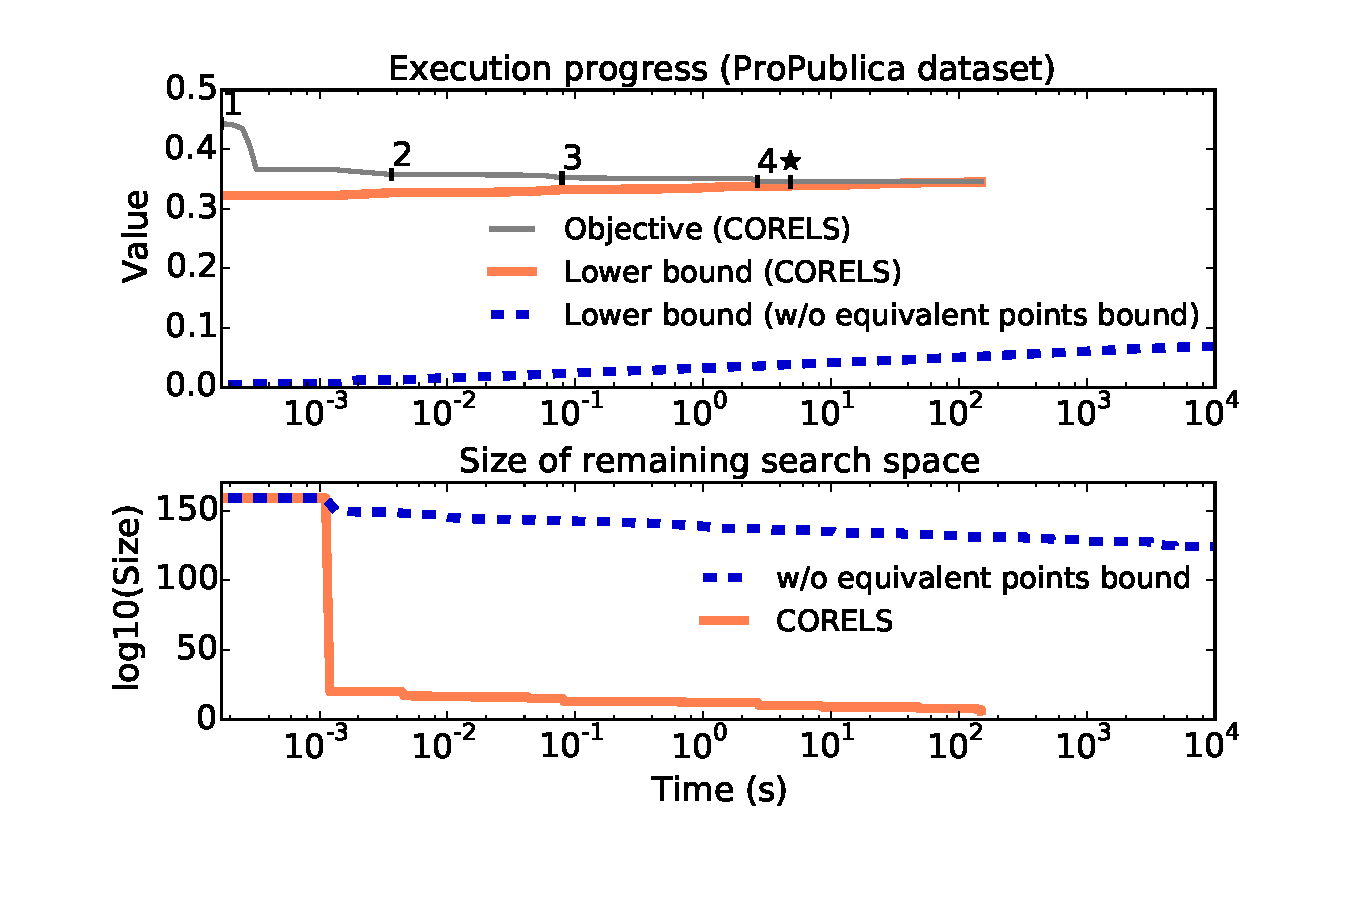
\includegraphics[trim={20mm, 15mm, 24mm, 15mm},
width=0.75\textwidth]{figs/compas_execution-remaining-space.pdf}
\end{center}
\caption{CORELS with (lines) and without
(dashes) the equivalent points bound (Theorem~\ref{thm:identical}).
%
Top: Objective value (thin line) and lower bound (thick line) for CORELS,
as a function of wall clock time (log scale).
%
Numbered hatch marks along the trace of the objective value
indicate when the length of the best known rule list changes,
and are labeled by the new length.
%
CORELS quickly achieves the optimal value (star marker),
and certifies optimality when the lower bound matches the objective value.
%
A separate execution of CORELS without the equivalent points bound remains
far from complete, and its lower bound (dashed line) far from the optimum.
%
Bottom: $\lfloor \log_{10} \Remaining(\CurrentObj, \Queue) \rfloor$,
as a function of wall clock time (log scale),
where~$\Remaining(\CurrentObj, \Queue)$
is the upper bound on remaining search space size
(Theorem~\ref{thm:remaining-eval-fine}).
}
\label{fig:objective}
\end{figure}

In the remainder, we show results using the ProPublica dataset.
%
The solid lines in Figure~\ref{fig:objective} illustrate how both the objective (top)
and the size of the remaining search space (bottom) decrease as CORELS executes.
%
The objective drops quickly, achieving the optimal value within 10 seconds.
CORELS certifies optimality in less than 6 minutes --
the objective lower bound of the remaining search space
steadily converges to the optimal objective as the search space shrinks.

Finally, we determine the efficacy of each of our bounds and data structure optimizations.
%
Both panels of Figure~\ref{fig:objective} also highlight a separate
execution of CORELS without the equivalent points bound.
%
After nearly 3 hours, the execution is still far from complete;
in particular, the lower bound is far from the optimum objective value.
%
Table~\ref{tab:ablation} provides summary statistics for experiments using the full
CORELS implementation and five variants that each remove a specific optimization.
%
Figure~\ref{fig:queue} presents a view of the same experiments.
%
%\includegraphics[width=0.75\textwidth]{figs/sketch-ablation.png}
\begin{table}[t!]
\centering
\begin{tabular}{l | c | c | c | c | c}
Removed component & $t_\text{total}$ (min) & $t_\text{opt}$ (s) & $i_\text{total}$ ($\times 10^6$) & $Q_\text{max}$ ($\times 10^6$) & $K_\text{max}$ \\
\hline
none (CORELS) & 5.5 (1.6) & 8 (2) & 1.7 (0.4) & 1.3 (0.4) & 5-6 \\
priority queue (BFS) & 6.7 (2.2) & 4 (1) & 1.9 (0.6) & 1.5 (0.5) & 5-6 \\
support bounds & 10.2 (3.4) & 13 (4) & 2.7 (0.8) & 2.2 (0.7) & 5-6 \\
symmetry-aware map & 58.6 (23.3) & 23 (6) & 16.0 (5.9) & 14.5 (5.7) & 5-6 \\
lookahead bound & 71.9 (23.0) & 9 (2) & 18.5 (5.9) & 16.3 (5.3) & 6-7 \\
%equiv. pts. bound & 188.6 (104.6) & 6178 (1840) & 803.8 (0.1) & 790.5 (0.4) & 10-10
equivalent pts bound & $>$134 & $>$7168* & $>$800 & $>$789 & $\ge$10
\end{tabular}
%\vspace{4mm}
\caption{Per-component performance improvement.
%
The columns report total execution time,
time to optimum, number of queue insertions,
maximum queue size, and maximum evaluated prefix length.
%
The first row shows CORELS; subsequent rows show variants
that each remove a specific implementation optimization or bound.
%
(We are not measuring the cumulative effects of removing a sequence of components.)
%
All rows represent complete executions, except for the final row,
in which each execution was terminated due to memory constraints,
once the size of the cache reached ${8 \times 10^8}$ elements,
after consuming 390-410GB RAM.
%
In all but the final row and column, we report means
(and standard deviations) over 10 cross-validation folds;
in the final row, we report the minimum values across folds. \\
%
*~Only 4 out of 10 folds achieve the optimum before being terminated.
}
\vspace{4mm}
\label{tab:ablation}
\end{table}
%
\begin{figure}[b!]
\begin{center}
% left lower right upper
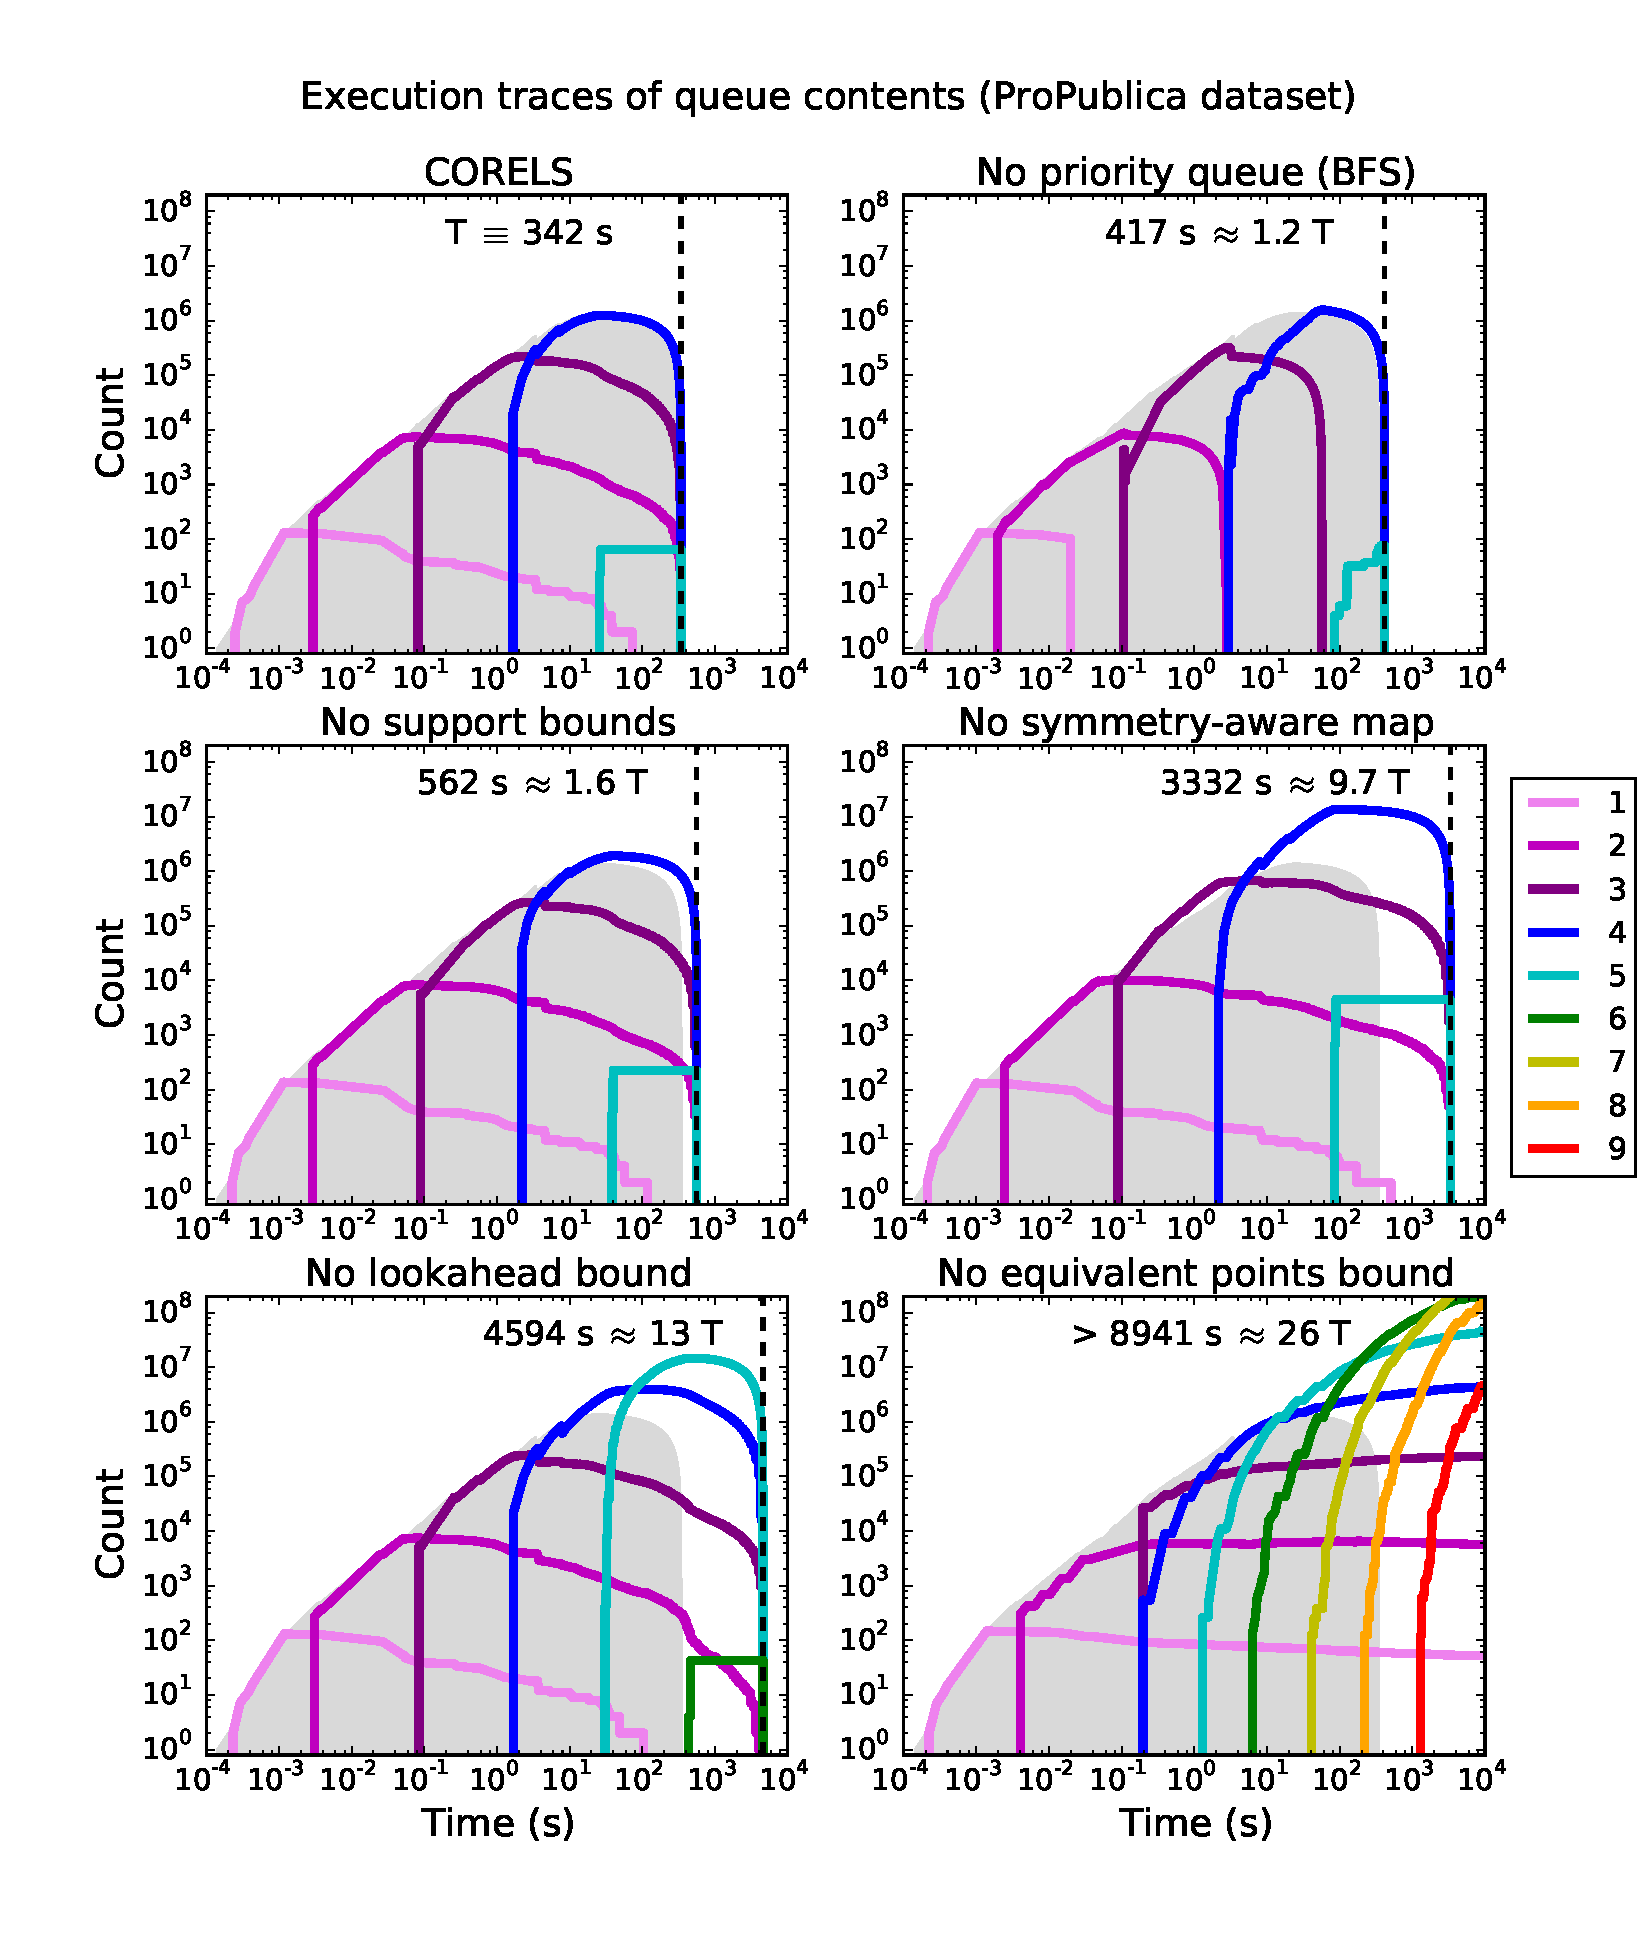
\includegraphics[trim={30mm 10mm 35mm 30mm},
width=0.85\textwidth]{figs/kdd_compas_ablation-queue.pdf}
\end{center}
\caption{Logical queue composition.
%
Numbers of prefixes in the queue (log scale), labeled and colored by length,
as a function of wall clock time (log scale), for full CORELS (top left),
and five variants that each remove a specific implementation optimization or bound.
%EXPAND HERE
%the permutation bounds (top right),
%lookahead bound (bottom left), and equivalent points bound (bottom right).
%
The gray shading fills in the area beneath the total number of
queue elements for CORELS,
\ie the sum over all lengths in the top left figure.
%
For comparison, we replicate the same gray region
in the other three subfigures.
%
For each execution, we indicate the total time both in seconds,
and relative to the full CORELS implementation (T = 149 s).
}
\label{fig:queue}
\end{figure}
%
These plots depict the number of prefixes of a given length in the queue
during the algorithm's execution.
